\section{Fundamentals}
\label{sec:fundamentals}

\begin{figure*}[t]
  \centering
  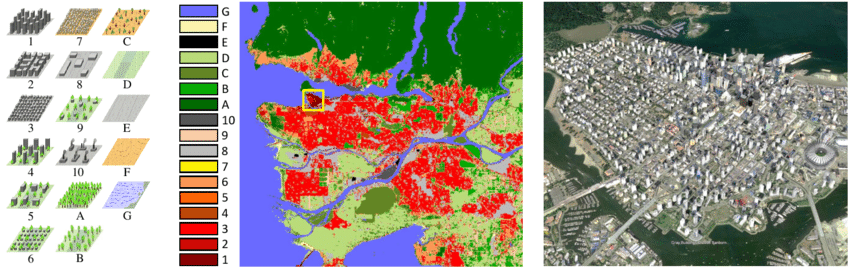
\includegraphics[width=0.9\linewidth]{images/schematic-lcz.png}
  \caption{The LCZ classes as schematics on the left and matching of classes for a city in the centre. Image taken from \cite{zhu_so2sat_2019}.}\label{fig:lcz_classes}
\end{figure*}


\subsection{Distributed Array Computation}
\label{subsec:distributed_array_computation}
Many scientific fields use \gls{numpy} as a basis for their calculation. Due to its implementation in the C language and its well designed
Python interface, the computation is fast and easy to write. But, \gls{numpy} arrays are only implemented for single node use.

Multiple libraries which allow the use of \gls{numpy} computations on multiple nodes have emerged: \cite{bauer_legate_2019}, \cite{huang_spartan_nodate}, \cite{krajsek_helmholtz_nodate}.
Noticeably, \cite{bauer_legate_2019} adds \gls{GPU} support to speedup specific operations e.g. big matrix calculations.

The hardest part in distributed array computing lies in the distribution of the data. All mentioned libraries provide
either the option to specify how the data should be distributed or even try to estimate the best distribution \cite{huang_spartan_nodate}.
All of them have a commonality in encapsulating and hiding the distribution of the data itself from the user.
This allows ease of use, but can lead to drops in performance when the user executes non optimal operations.


\subsection{MPI}
\label{subec:mpi}
\gls{MPI} is a message-passing standard published from the Message-Passing Interface Forum. It is currently available in version 3.1 \cite{message_passing_interface_forum_mpi_2015}.
\enquote{The goal of the Message-Passing-Interface \textelp{} is to develop a widely used standard for writing message-passing programs}\cite{message_passing_interface_forum_mpi_2015}.
\gls{MPI} is today widely used in \gls{HPC}, especially in Grid Computing. The standard interface allows to pass results or data between different processes or nodes.
Due to \gls{MPI} being a standard multiple implementations exist. Not all of the implementations are available for all systems and support all versions of the standard.
OpenMPI \cite{noauthor_open_nodate} and Intel MPI \cite{noauthor_intel_nodate} can be cited as examples, which are used in this work.
\gls{MPI} has some limitations that should be remembered when using it with big datasets. The most important limitation is the maximum message size, due to the size
being specified as an integer. Therefore, the maximum number of values that can be passed is \(2^{31} - 1\). Bigger messages need to be split in multiple messages or workarounds need to be implemented.

\subsection{HeAT}
\label{subsec:heat}
\gls{HeAT}, introduced in \cite{krajsek_helmholtz_nodate} is a mathematical library for distributed computations.
It conforms to a \gls{numpy} \cite{noauthor_numpy_nodate} interface and makes all distributed calculations transparent.
After executing \gls{HeAT} scripts single threaded during development, executing them parallel on a cluster is done by executing the same script with \gls{MPI}.
When used correctly, no changes to the code itself are necessary.
This is due to \gls{HeAT} wrapping \gls{PyTorch} as implementation with the correct \gls{MPI} synchronization to distribute the calculation.

To correctly perform the distributed calculation \gls{HeAT} adds a new data structure: the \gls{DNDarray}.
For a user accustomed to other libraries, the \gls{HeAT} API feels familiar, as it employs the general \gls{numpy} and \gls{PyTorch} tensor syntax
but introduces a split parameter.
The split parameter allows to control the axis, which the data is distributed across.
The developers decided to allow only one split axis to keep the development effort manageable.

Using the split parameter to control the distribution has some pitfalls for developers.
When reshaping or splicing the dataset one has to potentially rebalance the dataset. Additionally, this could incur communication effort
to redistribute the dataset across the nodes.
Other unexpected behavior especially for developers already having distributed computing experience is the need of all processes to call all \gls{HeAT} methods.
While in traditional \gls{MPI} one discriminates between the processes based on the rank, in \gls{HeAT} all nodes need to access all functions and \glspl{DNDarray} or the
program could lockup.

Furthermore, \gls{HeAT} provides the load utility for distributed loading of datasets. Through the usage of all nodes at the same time \gls{IO} is maximized and the data
is splitted already during loading. Therefore, calculations can start right away without the need to distribute the data
\cite{krajsek_helmholtz_nodate}.


\subsection{Local Climate Zone Classification}
\label{subsec:local_climate_zone_classification}

\glspl{LCZ} are a scheme formally proposed by \citeauthor{stewart_local_2012} in \cite{stewart_local_2012}. The scheme classifies areas based on fabric, land cover, structure
and metabolism into one of 17 \gls{LCZ}s \cite{xue_applications_2020}.
The \gls{LCZ}s are decided by 4 components:
\begin{enumerate}
  \item Height of roughness features
  \item Packing of roughness features
  \item Surface cover around roughness features
  \item Thermal admittance of materials
\end{enumerate}
The different classes can be seen in \cref{fig:lcz_classes}.
Suburban areas are complex and diverse which makes temperature and climate analysis hard to specify, therefor
\glspl{LCZ} were introduced to get more explainable and understandable divisions of those areas.
According to \citeauthor{stewart_local_2012}, the system fulfills all criteria of a logical local system as defined in \cite{grigg_logic_1965}.
Their work adds guidelines on how to classify an area correctly into their zones and how to use them afterwards.
These guidelines allow to keep a consistent labelling and create datasets with these labels.


\subsection{SO2Sat}
\label{subsec:so2sat}
\citeauthor{zhu_so2sat_2019} presented the SO2Sat dataset in \cite{zhu_so2sat_2019}.
They describe SO2Sat as a \enquote{valuable benchmark dataset \textelp{}, which consists of \gls{LCZ} labels of about half a million \textelp{} image patches}.
These images from the 42 different main cities are taken from the \gls{ESA} satellites Sentinel-1 and Sentinel-2. Each image is 32 by 32 pixels and contains 8 channels for Sentinel-1 and 10 channels for Sentinel-2.
After preprocessing these images they were given to domain experts for labelling which followed a \enquote{carefully designed labelling work flow} \cite{zhu_so2sat_2019}.
Through the careful work the dataset achieved a \enquote{overall confidence of 85\%} \cite{zhu_so2sat_2019}.
The labels consist of integers representing the 17 different \glspl{LCZ}.

\subsection{Spectral Clustering}
\label{subsec:spectral_clustering}

\begin{algorithm}[b]
  \SetKwData{Laplace}{\(L\)}\SetKwData{Adj}{\(W\)}
  \KwData{Similariy matrix \(S\), number \(k\) of clusters}
  \KwResult{Clusters \(A_1, \ldots, A_k\) }
  Construct a similarity graph\;
  \Adj \(\leftarrow\) weighted adjacency matrix\;
  \Laplace \(\leftarrow\) computeLaplacian(\Adj)\;
  \(u_1, \ldots, u_k \leftarrow\) computeEigenvectors(L)\;
  \(U\) \(\leftarrow\) Matrix with columns \(u_1, \ldots, u_k\)\;
  \ForEach(){\(i = 1, \ldots, n\)}{
    \(y_i\) \(\leftarrow\) vector corresponding to the \(i\)-th row of \(U\)
  }
\(C_1, \ldots, C_k \leftarrow\) kMeans(\(y_1, \ldots, y_n\))\;

  \caption{Basic Spectral Clustering}\label{alg:basic_spectral}
 \end{algorithm}

\enquote{Spectral clustering is the process of partitioning data samples into
\(k\) groups based on graph theory} \cite{krajsek_helmholtz_nodate}. Therefore,
to derive the formulation of Spectral Clustering we introduce the undirected graph \(G=(V, E)\) with nodes \(V\) and edges \(E\).
We consider the graph as weighted by assigning each edge a weight \(w_{ij}\). As the graph
is unidirectional, the weight is identical for \(w_{ij} = w_{ji} \).
% Degree Matrix
We define the degree of a vertex \(v_i \in V\) by iterating over all vertices \(v_j \in V\) that are connected to \(v_i\).
Therefore, the weight of the edge is positive:
\[d_i = \sum_{j=1}^n w_{ij}\]
Using the preceding definition, we set the degree matrix \(D\) as the diagonal matrix with the degrees \(d_1, \ldots, d_n\) on the diagonal.
\cite{von_luxburg_tutorial_2007}
% Weights Matrix
For two subsets of indices \(A, B\) we define the weights matrix \cite{von_luxburg_tutorial_2007}:
\[W(A, B) := \sum_{i \in A, j \in B} w_{ij}\]


The core element of spectral clustering is a similarity graph describing the similarity between different elements of the dataset.
There are several possible ways to construct a similarity graph fulfilling the mentioned criteria of an unidirectional graph.
The following three are used often for spectral clustering:
\begin{itemize}
  \item fully connected
  \item k-nearest neighbor
  \item \(\epsilon\)-neighborhood
\end{itemize}
The fully connected graph considers the similarity between all samples. The graph should model the local neighbors and is therefore only useful when the distance function
models the width of the neighborhood.
The k-nearest neighbor graph can be implemented in two ways. If we just use the definition of the k-nearest neighbors we would receive a directed graph.
To convert this into an undirected graph we can decide between connecting both vertices if one of them is a k-nearest neighbor of the other or connecting them if both vertices are nearest neighbors of each other.
The \(\epsilon\)-neighborhood graph only connects vertices whose similarity is smaller than \(\epsilon\).
Since this option already models the neighborhood directly, it usually is considered as an unweighted graph \cite{von_luxburg_tutorial_2007}.
According to \cite{von_luxburg_tutorial_2007} there is no theoretical work on the choosing of one method over
another.

Using the constructed similarity graph we need to calculate the spectrum of the similarity matrix.
This is done by constructing the normalized symmetric laplacian defined via
\[L_{sym} = I - D^{-1/2} W D^{-1/2}\]
using \(W, D\) as defined earlier.

The Lanczos algorithm \cite{lanczos_iteration_1950} is used to calculate the eigenvalues and eigenvectors from the laplacian.
When using the \(k\) smallest eigenvalues and the corresponding eigenvectors \(e_1, \ldots, e_k\) we can embed the dataset.

Now a clustering can be performed in the smaller embedding space of the eigenbasis using another algorithm, e.g. KMeans.
The overall algorithm can be found in algorithm \ref{alg:basic_spectral}.

\begin{figure}
  
\includegraphics{images/spectral_example.png}
  \caption{2 Half-Moon example for clustering performance of spectral clustering. Taken from \cite{noauthor_23_2020}.}
  \label{fig:spectral_example}
\end{figure}

One of the most common examples for spectral clustering can be seen in \cref{fig:spectral_example} \cite{noauthor_23_2020}. Spectral clustering is able to
separate the nonlinear datasets. This is often compared with KMeans which fails to correctly recognize the different clusters when using the euclidean distance.

\subsection{Distance Metrics}
\label{subsec:distance_metrics}
For spectral clustering the distance between samples needs to be measured. Depending on the data different ways to measure the distance are implemented in \gls{HeAT}.

\subsubsection{Euclidean Distance}
The euclidean distance is a well known way to measure the distance. The euclidean distance of two points \(X = (x_1, \ldots, x_n ), X' = (x_1', \ldots, x_n')\) is commonly defined  as:
\[
  d\left(X, X'\right) = \sqrt{{(x_1' - x_1)}^2 + \ldots + {(x_n' - x_n)}^2}
\]
It is fast and easy to calculate, but it is limited to  linear separation with most algorithms.

\subsubsection{Radial Basis Function Kernel}
\glspl{RBF} are a kernel that wrap the euclidean distance \(d\) \cite{vert_primer_2004}:
\begin{align*}
  \mathop{RBF} & \left(X, X'\right) = \exp(-\gamma d(X, X'))
\end{align*}
Where \(\gamma\) is a free parameter. An equivalent definition uses \(\gamma = \frac{1}{2\sigma^2}\), with a free parameter \(\sigma\).

The \glspl{RBF} are a measure of similarity and augment the effects of the euclidean distance due to the exponential function.
They allows to separate non-linear data with many algorithms.


\subsection{Clustering Evaluation Metrics}
\label{subsec:clustering_evaluation_metrics}

Evaluating clusters is more complicated than evaluating classification or other supervised machine learning tasks.
Unsupervised tasks can be evaluated using internal or external metrics.
While internal metrics, e.g. cluster purity, are derived from the result of the algorithm itself, external metrics are calculated from the comparison with given labels.
Since the in \cref{subsec:so2sat} explained dataset contains labels, this section is going to focus on external metrics.



\subsubsection{Adjusted Rand Index}
For the here presented metric we define \(C\) as the ground truth classes and \(K\) as the clustering assignment.
On this basis we define the following:\\
\(a\) - the number of pairs of elements that are in the same set in \(C\) and in the same set in \(K\)\\
\(b\) - the number of pairs of elements that are in different sets in \(C\) and in different sets in \(K\)\\
Then the \gls{RI} is mathematically given by \cite{noauthor_23_2020} as
\[RI = \frac{a + b}{C_2^{n_{samples}}}\]
When adjusting this index for random assignments we yield:
\[ARI = \frac{RI - \mathbb{E} [RI]}{\max (RI) - \mathbb{E} [RI]}\]
Both the \gls{ARI} and the \gls{RI} measure the similarity of two assignments.
While the \gls{RI} has problems with random assignments, the \gls{ARI} assigns a score close to \(0\)
to random assignments.


\subsubsection{V-Measure}
\label{ssec:v_measure}
The V-Measure was introduced by \citeauthor{rosenberg_v-measure_2007} in \cite{rosenberg_v-measure_2007} as an external clustering evaluation metric based on entropy.
The measurement is computed as a combination of homogenity and completeness. This allows the measurement to be explained more easily by logging homogenity and completeness additionally.
Homogenity measures if only data points of a single class are assigned to a single cluster. Completeness is defined symmetrically to homogenity by measuring if all data points of a single class are assigned to
a single cluster.
When combining these two with a parameter \(\beta\) we get the V-Measure \cite{noauthor_23_2020}:
\[v = \frac{(1 + \beta) \times \mathit{homogenity} \times \mathit{completeness}}{\beta \times \mathit{homogenity} + \mathit{completeness}}\]
Depending on the value of \(\beta\) we put more weight on homogenity or completeness. The usual value of \(\beta\) is \(1.0\) which weights both components equally.
The measurement is symmetric and bounded between \(0\) and \(1\), the later being the perfect achievable score.



\begin{figure*}
  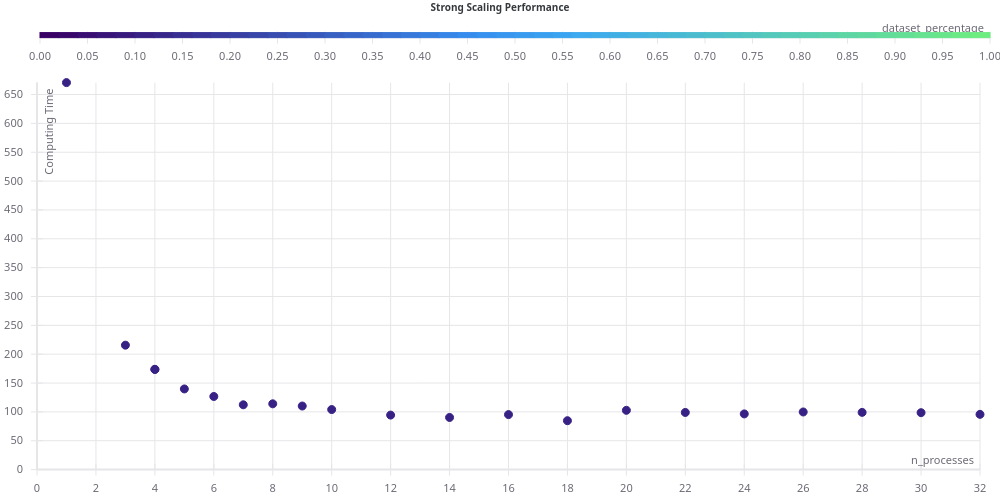
\includegraphics[width=0.9\linewidth]{images/strong_scaling_chart.png}
  \caption{Strong scaling behavior of the spectral clustering algorithm.}\label{fig:strong_scaling}
\end{figure*}
